%!TEX root = ../thesis.tex
\chapter{Appendix}

\section{Full-Sized Images}

\begin{figure}[h]
    \centering
    \begin{subfigure}[b]{0.45\textwidth}
        \centering
        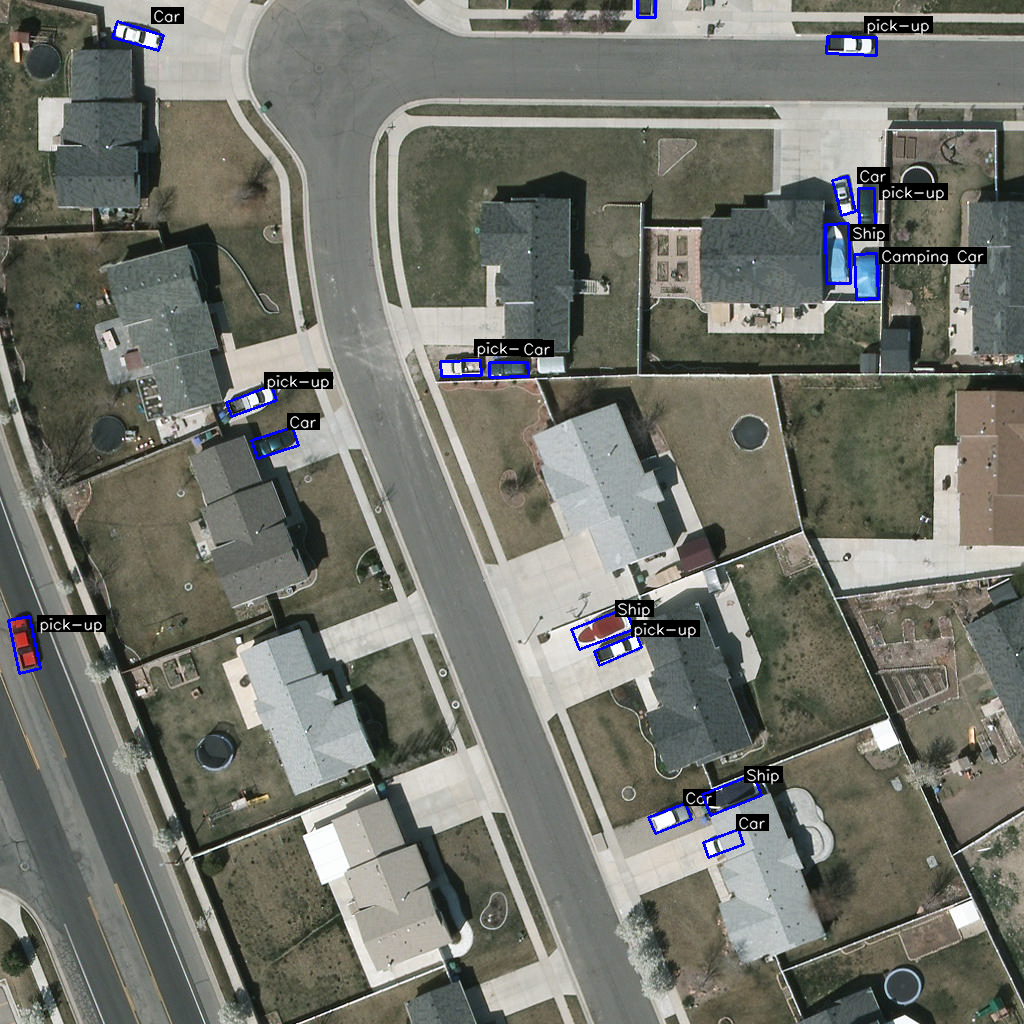
\includegraphics[width=\textwidth]{images/bb_smaller0.png}
        \caption{Two Coordinate out of range and smaller 0}
        \label{fig:smaller0_fs}
    \end{subfigure}
    \hfill
    \begin{subfigure}[b]{0.45\textwidth}
        \centering
        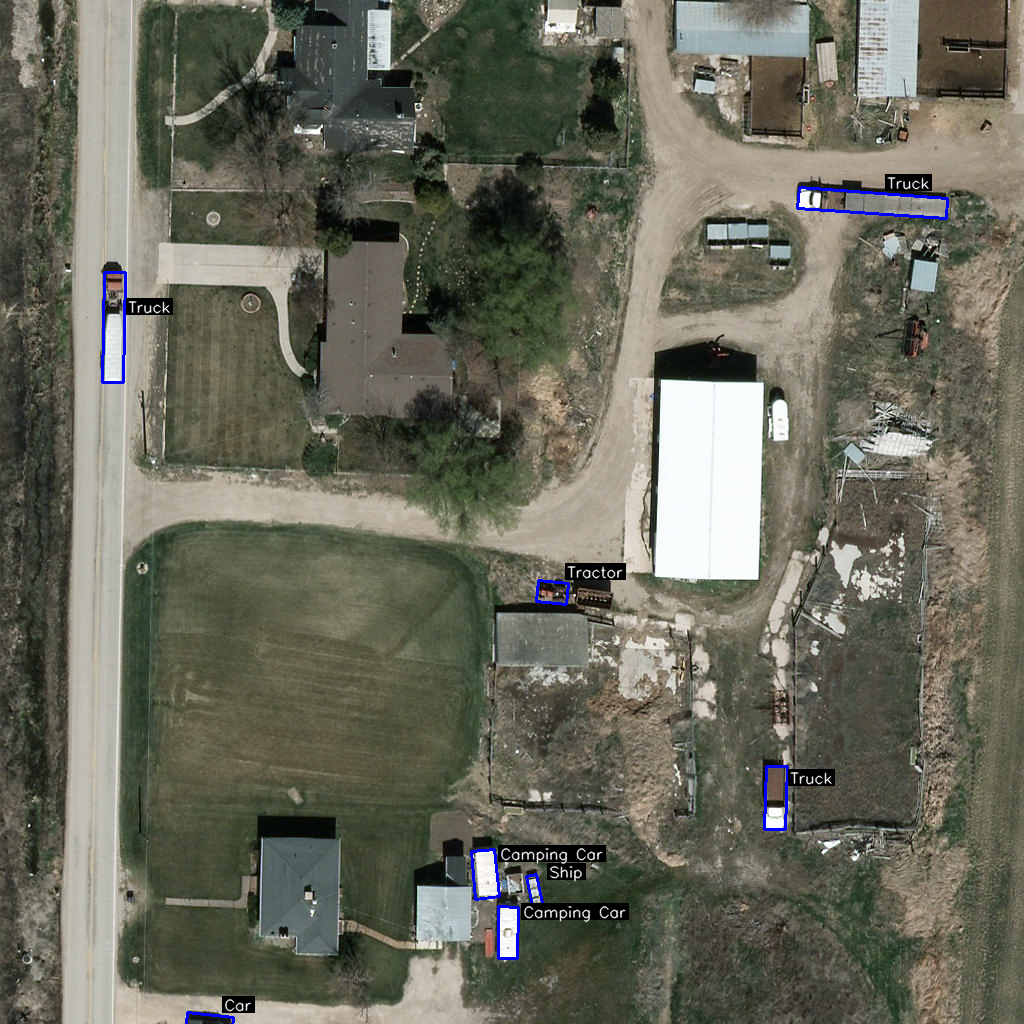
\includegraphics[width=\textwidth]{images/bb_higher1.png}
        \caption{Two Coordinates out ouf range and higher 1}
        \label{fig:higher1_fs}
    \end{subfigure}
    \caption{Example for label coordinates outside of the image (Full-Sized Image)}
    \label{fig:example_coords_ooR_fs}
\end{figure}


\begin{figure}[h]
    \centering
    
    % Erste Zeile
    \begin{subfigure}[b]{0.45\textwidth}
        \centering
        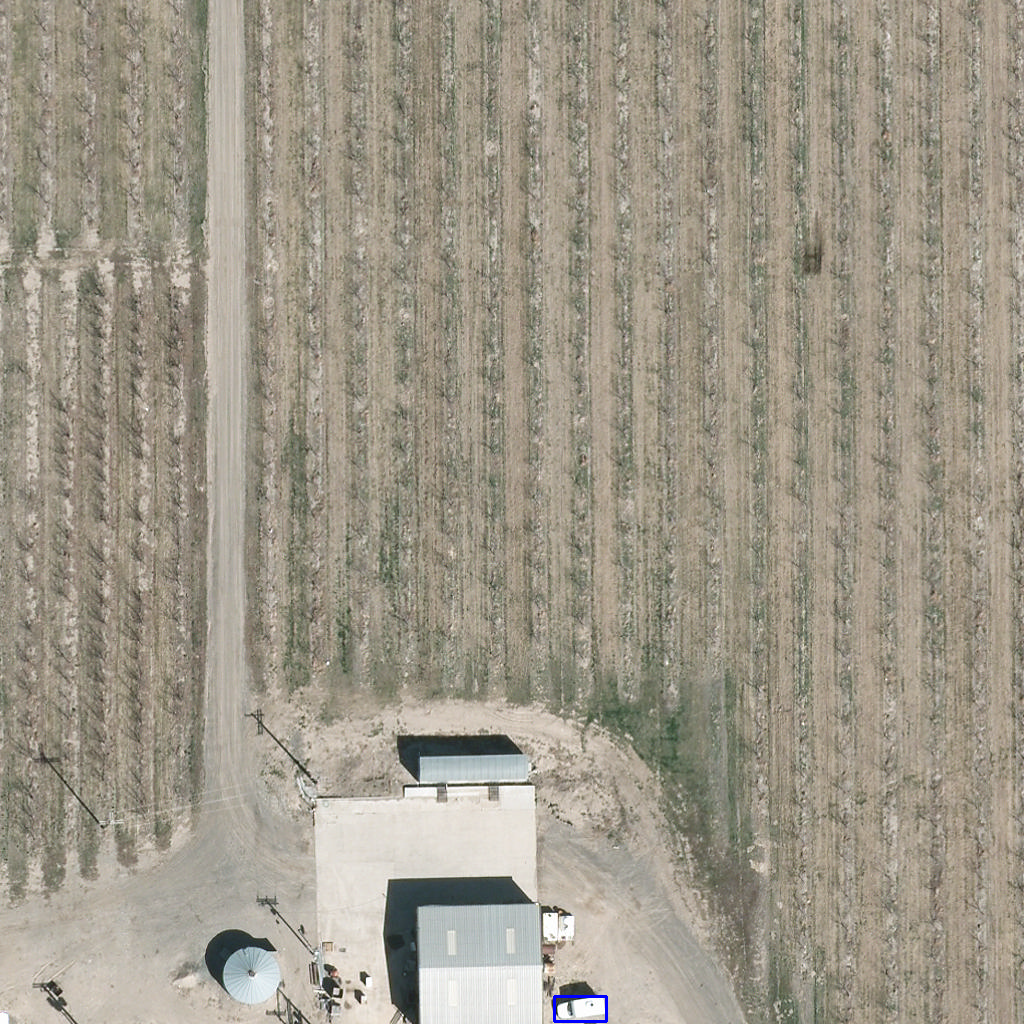
\includegraphics[width=\textwidth]{images/015Results/01abb_vs_obb/abb_truck.png}
        \caption{Label: "Truck", abb format, area: $\approx 1378 \text{px}$}
        \label{fig:abb_truck_fs}
    \end{subfigure}
    \hfill
    \begin{subfigure}[b]{0.45\textwidth}
        \centering
        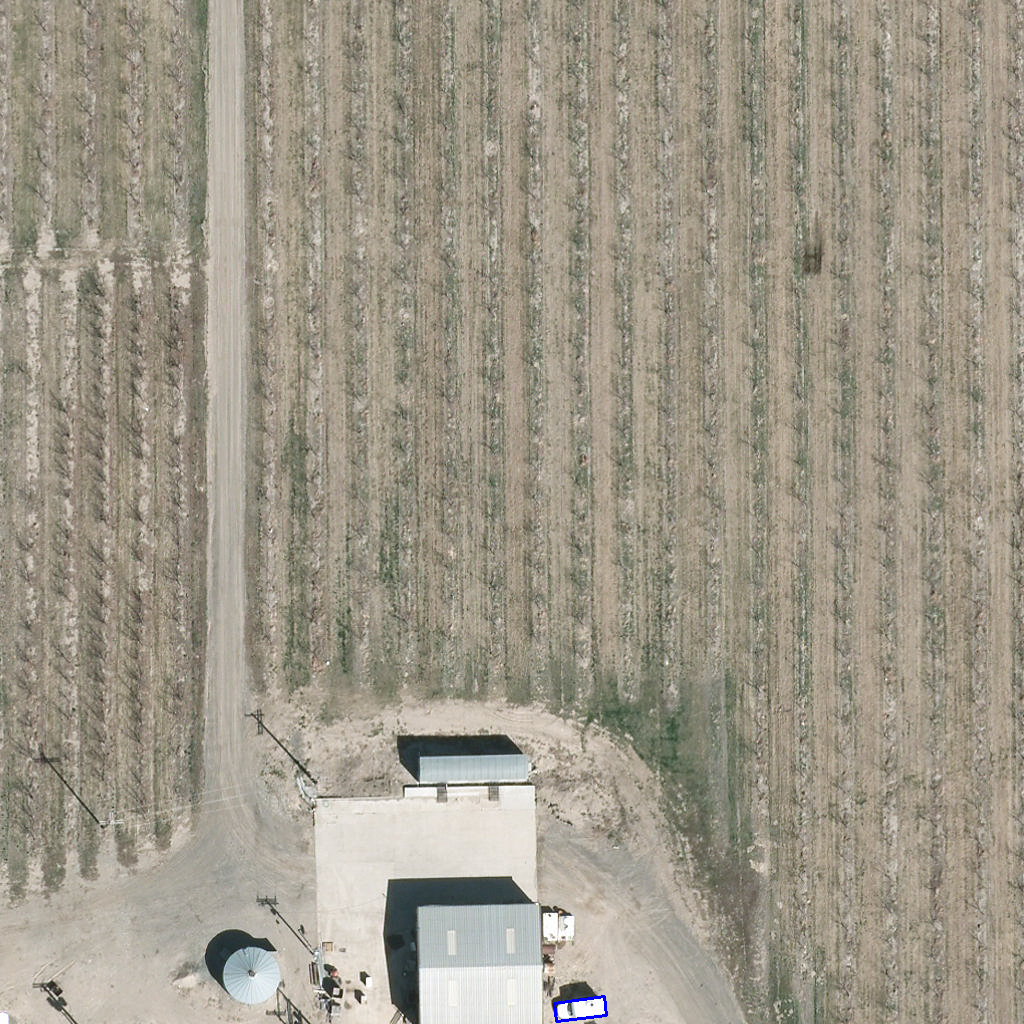
\includegraphics[width=\textwidth]{images/015Results/01abb_vs_obb/obb_truck.png}
        \caption{Label: "Truck", obb format, area: $\approx 967 \text{px}$}
        \label{fig:obb_truck_fs}
    \end{subfigure}
    
    \vspace{0.5cm} % Abstand zwischen den Zeilen
    
    % Zweite Zeile
    \begin{subfigure}[b]{0.45\textwidth}
        \centering
        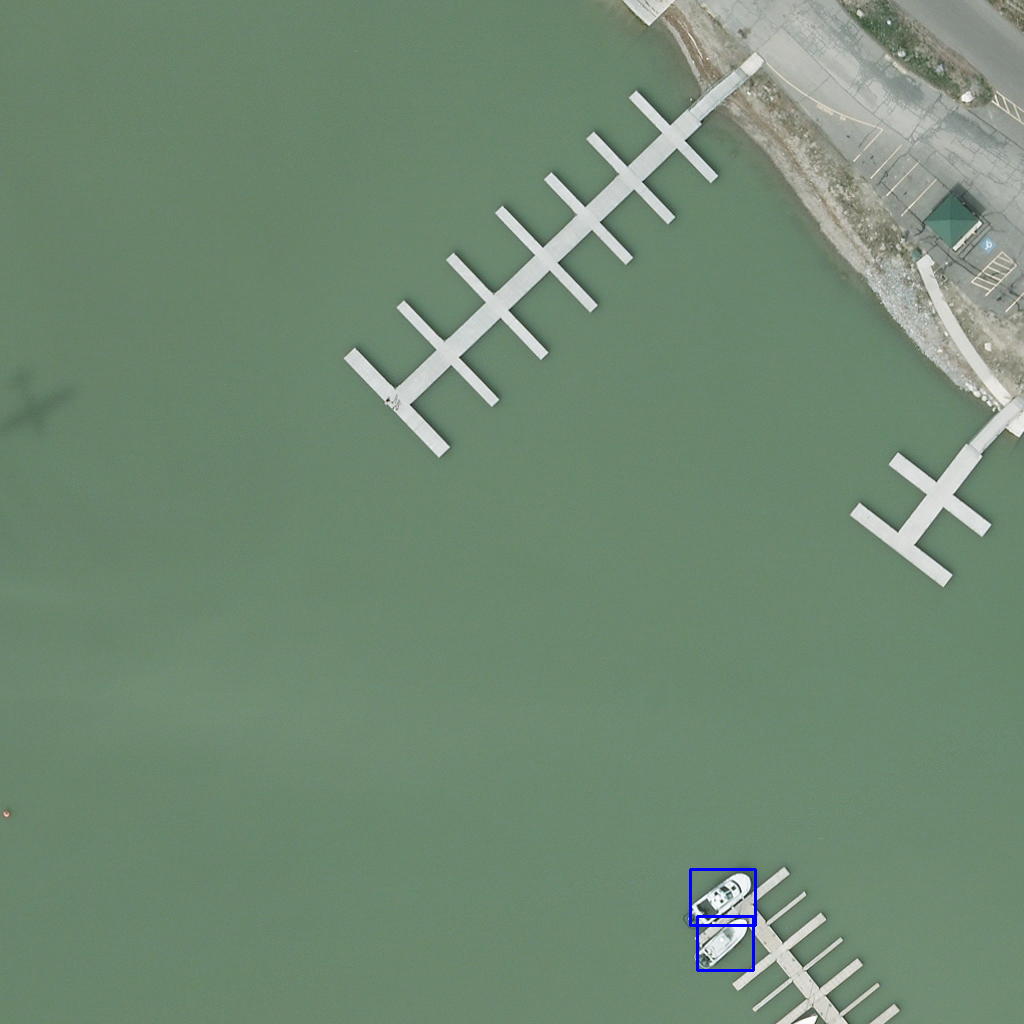
\includegraphics[width=\textwidth]{images/015Results/01abb_vs_obb/abb_ship.png}
        \caption{Labels: "Ship", abb format}
        \label{fig:abb_ship_fs}
    \end{subfigure}
    \hfill
    \begin{subfigure}[b]{0.45\textwidth}
        \centering
        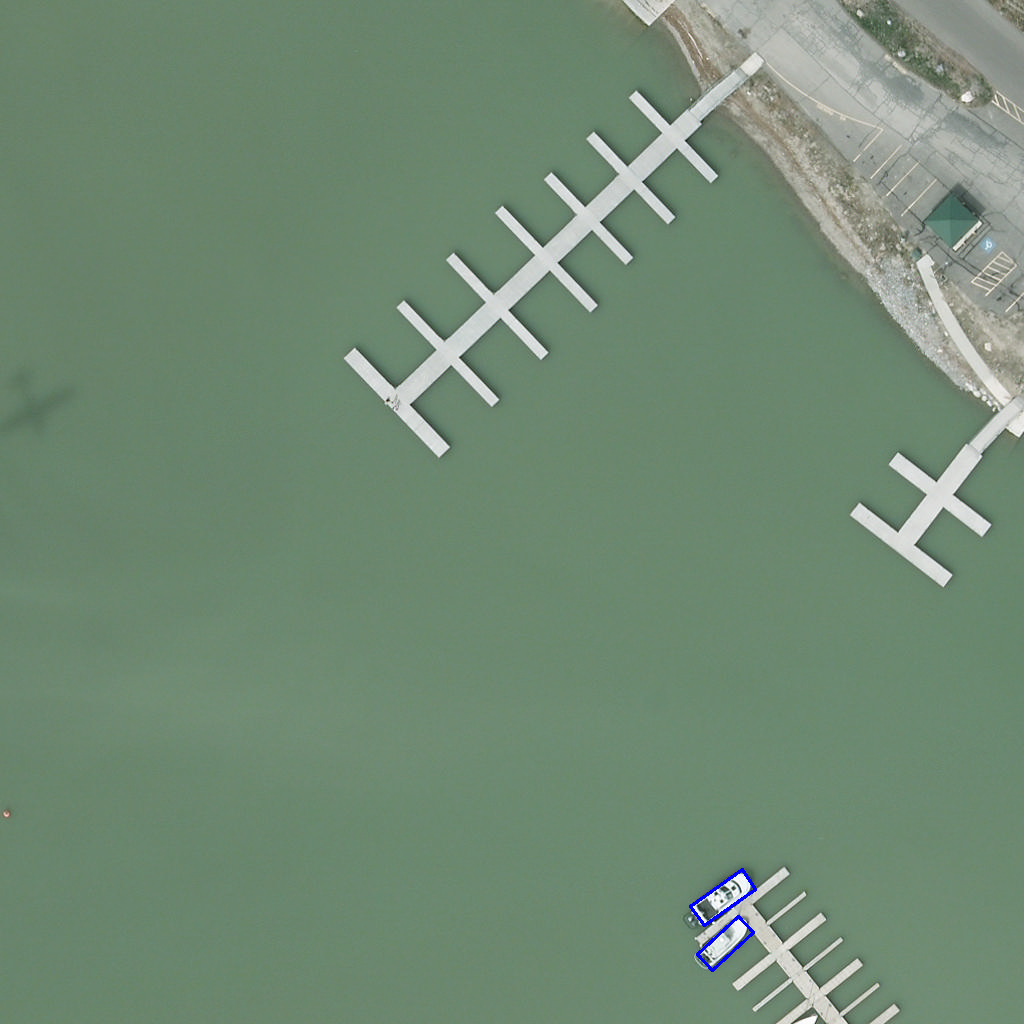
\includegraphics[width=\textwidth]{images/015Results/01abb_vs_obb/obb_ship.png}
        \caption{Labels: "Ship", obb format}
        \label{fig:obb_ship_fs}
    \end{subfigure}  
    \caption{Comparison of the bounding box formats of two different object classes (Full-Sized)}
    \label{fig:comparison_bb_format_fs}
\end{figure}

\clearpage

\section{Results}
\subsection{Calculation Bounding Box Area in Percent}
\label{ap:calc_bb_area_percent}

The total area of the image ($A_{\text{total}}$) is $1024 \times 1024 = 1,048,576 \text{ pixels}^2$.

\subsubsection*{Calculation of Bounding Box Area in Percent}
The percentage area ($F_{\%}$) is calculated using the following formula:
$$F_{\%} = \frac{A_{\text{Box}}}{A_{\text{total}}} \times 100\%$$

\subsubsection*{OBB (Oriented Bounding Box)}
The median area is $\approx 700$ pixels.
$$F_{\%,\text{obb}} = \frac{700}{1,048,576} \times 100\% \approx 0.06675\%$$

\subsubsection*{ABB (Axis-aligned Bounding Box)}
The median area is $\approx 1000$ pixels.
$$F_{\%,\text{abb}} = \frac{1000}{1,048,576} \times 100\% \approx 0.09536\%$$